\documentclass[11pt,aspectratio=169]{beamer}
%%%%%%%%% GENERAL PACKAGES
%\usepackage[dvipsnames]{xcolor}
%\usepackage{pdfpages}
%\usetheme[progressbar=frametitle]{metropolis}
%\setbeamercolor{background canvas}{bg=white}
%\usepackage{appendixnumberbeamer}
%\usepackage{booktabs}
%\usepackage[scale=2]{ccicons}
%\usepackage{pgfplots}
%\usepgfplotslibrary{dateplot}
%\usepackage{xspace}
%\newcommand{\themename}{\textbf{\textsc{metropolis}}\xspace}
%\usepackage[absolute,overlay]{textpos}






%%%%%%%%% COLOR THEME

% Define some colors:
\definecolor{DarkFern}{HTML}{407428}
\definecolor{DarkCharcoal}{HTML}{4D4944}
\definecolor{AlertColor}{RGB}{89,124,158}
\definecolor{HighLight}{RGB}{96,95,134}
\definecolor{Important}{RGB}{234,122,133}
\definecolor{Yellow}{HTML}{00539C}
\colorlet{Fern}{DarkFern!85!white}
\colorlet{Charcoal}{DarkCharcoal!85!white}
\colorlet{LightCharcoal}{Charcoal!50!white}
\colorlet{HighLight2}{AlertColor}
\colorlet{DarkRed}{red!70!black}
\colorlet{DarkBlue}{blue!70!black}
\colorlet{DarkGreen}{green!70!black}
\definecolor{RoyalBlue}{HTML}{00539C}
\definecolor{Peach}{HTML}{EEA47F}
\definecolor{ForestGreen}{HTML}{2C5F2D}
\definecolor{MossGreen}{HTML}{E8FCC9}
\definecolor{SeaGreen}{HTML}{2E8B57}
% Use the colors:
\setbeamercolor{title}{fg=Fern}
\setbeamercolor{frametitle}{fg=MossGreen,bg=ForestGreen}
\setbeamercolor{normal text}{fg=Charcoal!70!black}
\setbeamercolor{block title}{fg=black,bg=Fern!25!white}
\setbeamercolor{block body}{fg=black,bg=Fern!10!white}
\setbeamercolor{block title alerted}{fg=black,bg=DarkRed!25!white}
\setbeamercolor{block body alerted}{fg=black,bg=DarkRed!10!white}
\setbeamercolor{alerted text}{fg=DarkRed}
\setbeamercolor{itemize item}{fg=Charcoal}



%%%%%%%%% OTHER COMMANDS
\newcommand{\indep}{\perp\!\!\! \perp}
\newcommand{\comment}[1]{}
\newcommand{\bs}{\boldsymbol}
\newcommand{\tr}{\text{trace}}
\newcommand{\sgn}{{\rm sgn}}
\def\T{\top}
%\newcommand{\det}{\text{det}}
\newcommand{\var}{\mathrm{var}}
\newcommand{\cC}{{\cal C}}
\renewcommand{\d}{{\rm d}}
\newcommand{\cG}{{\cal G}}
\newcommand{\cV}{{\cal V}}
\newcommand{\cE}{{\cal E}}
\newcommand{\cM}{{\cal M}}
\newcommand{\cP}{{\cal P}}
\newcommand{\cX}{{\cal X}}
\newcommand{\cY}{{\cal Y}}
\newcommand{\X}{\mathbf{X}}
\newcommand{\Y}{\mathbf{Y}}
\newcommand{\x}{\mathbf{x}}
\newcommand{\y}{\mathbf{y}}
\newcommand{\z}{\mathbf{z}}

\newcommand{\argmin}{\operatornamewithlimits{argmin}}
\newcommand{\eps}{\varepsilon}
\newcommand{\<}{\langle}
\renewcommand{\>}{\rangle}


%

\setbeamertemplate{navigation symbols}{}
\setbeamertemplate{footline}[text line]{%
    \hfill\strut{%
        \scriptsize\sf\color{black!60}%
        \quad\insertframenumber/\inserttotalframenumber
    }
    %\hfill
    }


\usenavigationsymbolstemplate{}
\setbeamersize{text margin left=.2cm,text margin right=.2cm} 
\addtobeamertemplate{frametitle}{}{\vspace{-1.2mm}}
\setbeamertemplate{itemize item}{$\bullet$}

\setbeamertemplate{itemize subitem}{\tiny\raise1.5pt\hbox{\donotcoloroutermaths$\blacktriangleright$}}
\setbeamertemplate{itemize subsubitem}{\tiny\raise1.5pt\hbox{\donotcoloroutermaths$\blacktriangleright$}}
\setbeamertemplate{enumerate item}{\insertenumlabel.}
\setbeamertemplate{enumerate subitem}{\insertenumlabel.\insertsubenumlabel}
\setbeamertemplate{enumerate subsubitem}{\insertenumlabel.\insertsubenumlabel.\insertsubsubenumlabel}
\setbeamertemplate{enumerate mini template}{\insertenumlabel}






\newcommand{\TODO}[1]{{\color{red}{[TODO: #1]}}}


\newcommand{\R}{\mathbb R}
\newcommand{\E}{\mathbb E}
\renewcommand{\P}{\mathbb P}


\DeclareMathOperator*{\cov}{cov}


\newsavebox{\zerobox}
\newenvironment{nospace}
{\par\edef\theprevdepth{\the\prevdepth}\nointerlineskip
  \setbox\zerobox=\vtop to 0pt\bgroup
  \hrule height0pt\kern\dimexpr\baselineskip-\topskip\relax
}
{\par\vss\egroup\ht\zerobox=0pt \wd\zerobox=0pt \dp\zerobox=0pt
  \box\zerobox}

\usepackage{soul}
\makeatletter
\let\HL\hl
\renewcommand\hl{%
  \let\set@color\beamerorig@set@color
  \let\reset@color\beamerorig@reset@color
  \HL}
  \makeatother



%\usecolortheme{whale}

\title[Calculus and Linear Algebra]{Lecture 4: Calculus and Linear Algebra}
\author[Piotr Zwiernik, Barcelona School of Economics]{Piotr Zwiernik \\ $\;$\\
Mathematics Brush-up\\ $\;$\\ $\;$\\

\includegraphics[width=1.5in]{img/bse.png}  
}
\date{}

%\beamerdefaultoverlayspecification{<+->}

\begin{document}
\begin{frame}
\titlepage
\end{frame}


\begin{frame}
\frametitle{Chapter 9: Functions of several variables}
\begin{small}
In many economic applications, we have to deal with situations where \textcolor{blue}{several variables} have to be included in the mathematical model. 
\vskip 12pt
\textcolor{blue}{Example}: The \textcolor{blue}{Cobb-Douglas production function} applied to an agricultural production gives the number of units produced depending on the capital invested, the labour and the area of land used for the production.
\vskip 12pt
\textcolor{blue}{Read}  Chapter 11 of Werner-Sotskov and Chapters 14 and 17 of Simon-Blume
\vskip 12pt
\textcolor{blue}{Exercises:} 11.11 a), 11.21, 11.22 (Werner-Sotskov)


\end{small}
\end{frame}



\begin{frame}
\frametitle{Definition}
\begin{small}
A \textcolor{blue}{function of several variables} is a map $f: D \rightarrow \R$ where $D \subset \R^n$ is the domain, and for any point $(x_1,\dots,x_n)\in D$ it assigns a number
$f(x_1,\dots,x_n)$.

\begin{tiny}We can only plot $n=2$!\end{tiny}
\vskip 10pt
If $n=2$, the graph of $f$ with $z=f(x,y)$ is called a \textcolor{blue}{surface} and it is plotted in $\R^3$.
\vskip 12pt
If $n=2$ a \textcolor{blue}{level curve} of $f$ is a curve in $\R^2$ given by $$z=f(x,y)=C.$$





\end{small}
\end{frame}



\begin{frame}
\frametitle{Example}
\begin{small} $f(x,y)=100-x^2-y^2$\end{small} \begin{tiny}the surface is a smooth cone and the level curves are circles centered at zero\end{tiny}
\begin{figure}
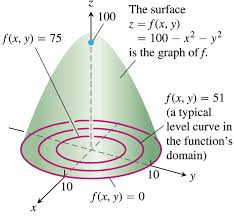
\includegraphics[width=2.5in]{img/level_curve} 
\end{figure}
\end{frame}

\begin{frame}
\frametitle{Economic example}
\begin{small}
 \textcolor{blue}{Cobb-Douglas production function} $$P(L,K)=b L^{\alpha} K^{\beta}$$
 \begin{tiny}$P$ is the total production, $L$ is the labor, $K$ the capital, $b$ the total factor productivity, and $\alpha$ and $\beta$ are the output elasticities of labor and capital, respectively. The parameters $b$, $\alpha$ and $\beta$ are constants computed by available technology. \end{tiny}
 
 The domain is 
$D=\{(L,K) \in \R^2: L \geq 0, K \geq 0\}$.
\end{small}
\begin{figure}
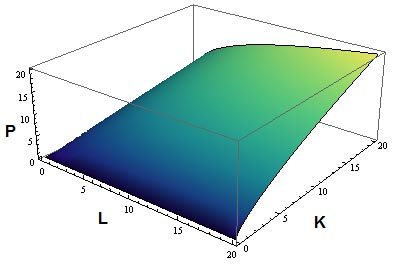
\includegraphics[width=2.5in]{img/cd.jpg} 
\end{figure}
\end{frame}

\begin{frame}
\frametitle{Cobb-Douglas production function}
\begin{small}
The  parameters  $\alpha$, and $\beta$ measure the \textcolor{blue}{output change} in  levels of labor or capital change. For example, if $\alpha=0.15$, a $1\%$ increase in  labor would lead to approximately a $0.15\%$ increase  in output.
 \vskip 12pt
 If $\alpha+\beta=1$, the  production function has  \textcolor{blue}{constant returns to scale} (the  output increases by the same proportional change). That is, if  $L$ and $K$ each increase by  $20\%$, then $P$ increases  by $20\%$.
 \vskip 12pt
 If $\alpha+\beta<1$, the returns to scale are \textcolor{blue}{decreasing}.
 \vskip 12pt
 If $\alpha+\beta>1$,  the returns to scale are \textcolor{blue}{increasing}.
 
\end{small}

\end{frame}

\begin{frame}
\frametitle{Multivariate Gaussian density}
\begin{small}
 A random vector ${\bf X}$ in $\R^d$ has a 
 \textcolor{blue}{multivariate Gaussian distribution}
 with a nonsingular covariance matrix $\Sigma$ if $\Sigma$ is positive definite and the density function of $X$ is
 $$
 f({\bf x})=(2 \pi)^{-d/2} \text{det}(\Sigma)^{-1/2} \exp \left(
-\frac12 ({\bf x}-{\bf m})' \Sigma^{-1} ({\bf x}-{\bf m})\right)
 $$
 where ${\bf x} \in \R^d$, ${\bf m}=E({\bf X})$, and 
 $$
 \Sigma=E(({\bf X}-{\bf m})({\bf X}-{\bf m})').
 $$
\end{small}
\end{frame}

\begin{frame}
\frametitle{Multivariate Gaussian density}
\begin{small}
\textcolor{blue}{Example:} $d=2$, ${\bf m}={\bf 0}$, $\sigma_1^2=1$, $\sigma_2^2=4$
\end{small}
\begin{figure}
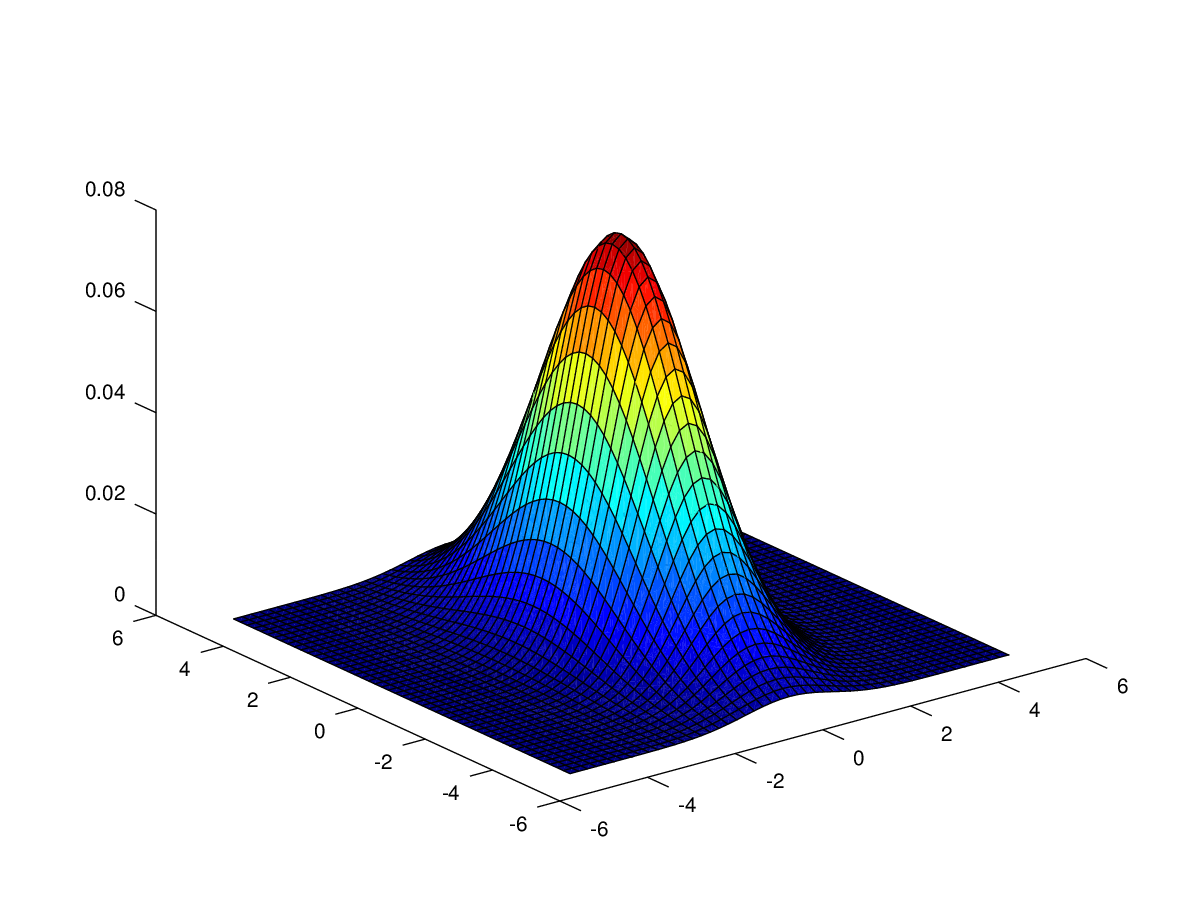
\includegraphics[width=3in]{img/multiv} 
\end{figure}
\end{frame}

\begin{frame}
\frametitle{Partial derivatives}
\begin{small}
A function $f: D \subset\R^2 \rightarrow \R$ is \textcolor{blue}{partially differentiable} with respect to $x$ at $(x,y)$ if the limit
$$
\lim_{h\rightarrow 0} \frac{f(x+h,y)-f(x,y)}{h} \qquad \text{exists},
$$
and is \textcolor{blue}{partially differentiable} with respect to $y$ at $(x,y)$ if the limit
$$
\lim_{h\rightarrow 0} \frac{f(x,y+h)-f(x,y)}{h} \qquad \text{exists}.
$$
Both limits are called the \textcolor{blue}{partial derivatives} of $f$ with respect to $x$ and $y$ and denoted $f_x(x,y)$, $f_y(x,y)$ or 
$\frac{\partial f(x,y)}{\partial x} $, $\frac{\partial f(x,y)}{\partial y}$.
\vskip 10pt
\textcolor{blue}{Example:} Total cost of a firm producing $x$ units of product $A$ and $y$ units of product $B$ is
$$
C(x,y)=200+22x+16y^{3/2}.
$$ 
\textcolor{blue}{Marginal costs:} $C_x(x,y)=22, C_y(x,y)=24 \sqrt{y}$.


\end{small}
\end{frame}


\begin{frame}
\frametitle{Cobb-Douglas production function}
\begin{small}
The partial derivative $\frac{\partial P}{\partial L}$ is the rate at  which production changes with respect to the amount of labor. It is called the \textcolor{blue}{marginal productivity of labor}.
 \vskip 10pt
 The partial derivative $\frac{\partial P}{\partial K}$ is the rate at  which production changes with respect to the amount of capital. It is called the \textcolor{blue}{marginal productivity of capital}.
 \vskip 10pt
 The \textcolor{blue}{assumptions}  made by Cobb and Douglas are:
 \begin{enumerate}
\item  If either labor or capital vanish then so will the  production.
\item The marginal productivity of labor is \textcolor{blue}{proportional} to the  amount  of production per unit of labor, that is,
$$
\frac{\partial P}{\partial L}=\alpha \frac{P}{L} \quad \text{ for some }  \alpha.
$$
\item The marginal productivity of capital is \textcolor{blue}{proportional} to the  amount  of production per unit of capital, that is,
$$
\frac{\partial P}{\partial K}=\beta \frac{P}{K}\quad \text{for some } \beta.
$$
\begin{tiny}(In Chapter 10 we will show that these assumptions imply that $P=b L^{\alpha} K^{\beta}$) \end{tiny}
 \end{enumerate}
 
\end{small}

\end{frame}

\begin{frame}
\frametitle{Tangent plane and total derivative}
\begin{small}
\textcolor{blue}{Geometric interpretation:} $f_x(x_0,y_0)$ (resp.   $f_y(x_0,y_0)$) is the slope of the tangent line $f_T(x)$ to the curve of intersection of the surface $z=f(x,y)$ and the plane $y=y_0$ (resp. $x=x_0$) at $(x_0,y_0,z_0)$, where $z_0=f(x_0, y_0)$.
\vskip 12pt
 Both tangent lines $f_T(x)$ and $f_T(y)$ span a plane $f_T(x,y)$ which is called the \textcolor{blue}{tangent plane} to $z=f(x,y)$ at $(x_0,y_0,z_0)$, and the equation of the tangent plane is
$$
f_T(x,y)=f(x_0,y_0)+f_x(x_0, y_0) (x-x_0) +f_y(x_0, y_0) (y-y_0).
$$

\vskip 12pt
 The tangent plane gives and approximation of the total change of the function from $(x_0, y_0)$ to $(x,y)$, when both points are close:
$$
f(x,y)-f(x_0,y_0)\approx f_x(x_0, y_0) (x-x_0) +f_y(x_0, y_0) (y-y_0),
$$
which can be seen as a \textcolor{blue}{total derivative}. In differential notation:
$$
df= f_x(x_0, y_0) dx +f_y(x_0, y_0) dy.
$$


\end{small}
\end{frame}


\begin{frame}
\frametitle{Tangent plane}
\begin{figure}
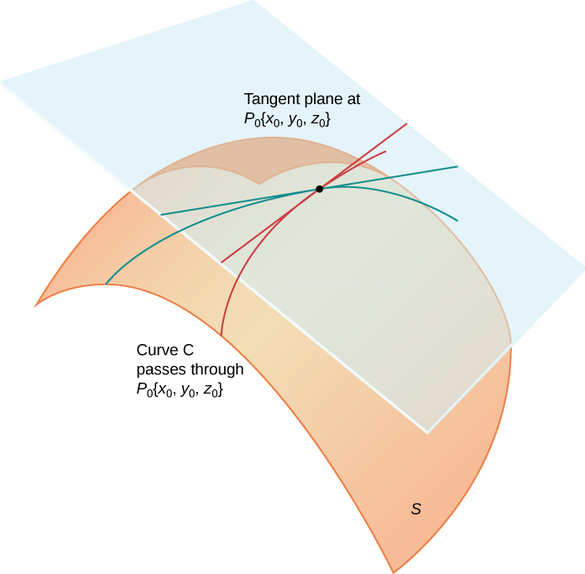
\includegraphics[width=3in]{img/tp.jpg} 
\end{figure}
\end{frame}




\begin{frame}
\frametitle{Higher Partial derivatives}
\begin{small}
We can consider \textcolor{blue}{higher-order partial derivatives} of $f:D \subset \R^n \rightarrow \R$, when they exists. For example
$$
f_{xy}(x,y)=\frac{\partial}{\partial y} \left( \frac{\partial f(x,y)}{\partial x}\right)=
\frac{\partial^2 f(x,y)}{\partial y \partial x}.
$$ 
\vskip 12pt
 \textcolor{blue}{Theorem (Young):} If $f_{xy}$ and $f_{yx}$ are continuous, they coincide.
\vskip 12pt
 \textcolor{blue}{Example:} $f(x,y)=\sin(3x-y)$, $f_{xy}=f_{yx}=3 \sin(3x-y)$.


\end{small}
\end{frame}
\begin{frame}
\frametitle{The gradient}
\begin{small}
Let ${\bf x}=(x_1,\ldots,x_n) \in D$.The vector
$$
\nabla f({\bf x})=(f_{x_1}({\bf x}),\dots,f_{x_n}({\bf x})).
$$
is called the \textcolor{blue}{gradient} of $f$ at ${\bf x}$, when all partial derivatives exist.
\vskip 10pt

 \textcolor{blue}{Example:} $f(x,y)=2x^2+\frac12 y^2$, $\nabla f(x,y)=(4x, y)$, 
$\nabla f(1,2)=(4, 2)$ 

\vskip 10pt
 The gradient gives the direction which the function $f$ at ${\bf x}$ \textcolor{blue}{increases the most}, since it is orthogonal to the tangent line to the level curve at this point.
\vskip 10pt

 \textcolor{blue}{Example:} production function: $f(x,y)=3x^2y+0.5 x e^y$, $x=$labour, $y=$capital,
$\nabla f(x,y)=(6xy+0.5 e^y, 3x^2+0.5xe^y)$
\vskip 10pt
$\nabla f(10,\log 12)=(155.09, 360)$, so to increase at maximum the production, the firm should increase labour and capital in the ratio $155.09:360$, that is, if we increase the labor by 1 we increase the capital by 2.32.


\end{small}
\end{frame}

\begin{frame}
\frametitle{Example: $f(x,y)=2x^2+\frac12 y^2$}
\begin{small}$\nabla f(x,y)=(4x, y)$, $\nabla f(1,2)=(4, 2)$, therefore the maximum direction of increase at point $(1,2)$ is the direction $(4,2)$. 
\vskip 10pt
The point $(1,2)$ is at the level curve $2x^2+\frac12y^2=4$.\end{small}
\begin{figure}
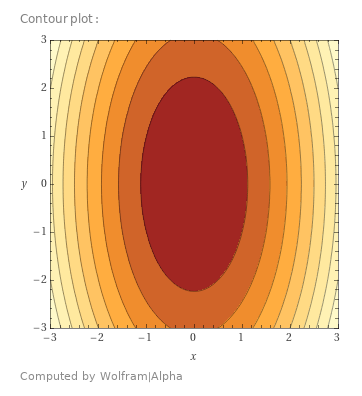
\includegraphics[width=2in]{img/level_ex} 
\end{figure}
\end{frame}

\begin{frame}
\frametitle{Differentiation rules for matrices}
\begin{small}
Consider two vectors ${\bf x}=(x_1,...,x_n)$ and ${\bf y}=(y_1,...,y_m)$ in $\R^n$ and $\R^m$, respectively, where each $y_i$ depends on ${\bf x}$. Then we denote by $
\frac{d {\bf y}}{d {\bf x}}$
the Jacobian $m \times n$ matrix with entries $\frac{\partial y_i}{\partial x_j}$.

\begin{tiny} If $m=1$, then the Jacobian is just the gradient.\end{tiny}

\vskip 12pt
\textcolor{blue}{Examples:}

\begin{enumerate}
\item If $A$ is a $m \times n$ matrix, then
$$
\frac{d (A {\bf x})}{d{\bf x}}=A
$$

\begin{tiny} If $m=1$ the we deduce that $\frac{d ({\bf a}'{\bf x})}{d{\bf x}}={\bf a}$.\end{tiny}

\item If $A$ is a $n \times n$ matrix, then
$$
\frac{d ({\bf x}'A{\bf x})}{d{\bf x}}={\bf x}'(A+A').
$$
\end{enumerate}
\end{small}
\end{frame}

\begin{frame}
\frametitle{Unconstrained optimization}
\begin{small}
A function $f:D \subset \R^n \rightarrow \R$ has a \textcolor{blue}{local max} (\textcolor{blue}{min})
at ${\bf x}_0$ if there exists a ball $B_r({\bf x_0})\subset D$ such that
$$
f({\bf x}) \leq f({\bf x}_0) \qquad (f({\bf x}) \geq f({\bf x}_0) )
$$
for all ${\bf x} \in B_r({\bf x}_0)$. If the inequality holds for all ${\bf x} \in D$, we say it is a \textcolor{blue}{global max} (\textcolor{blue}{min}).
\vskip 10pt
We say that ${\bf x}$ is an \textcolor{blue}{interior point} if there exists a ball $B_r({\bf x})\subset D$.
\vskip 10pt
 \textcolor{blue}{Theorem (Necessary 1st order condition):} If $f$ has a local max or min at ${\bf x}$ and it is an interior point then $\nabla f ({\bf x})={\bf 0}$.
\vskip 10pt
 Interior points ${\bf x}$ that $\nabla f ({\bf x})={\bf 0}$ are called \textcolor{blue}{stationary points}. 
\vskip 10pt
 Stationary points that are neither a local max or min are called \textcolor{blue}{saddle points}.


\end{small}
\end{frame}

\begin{frame}
\frametitle{Unconstrained optimization}
\begin{figure}
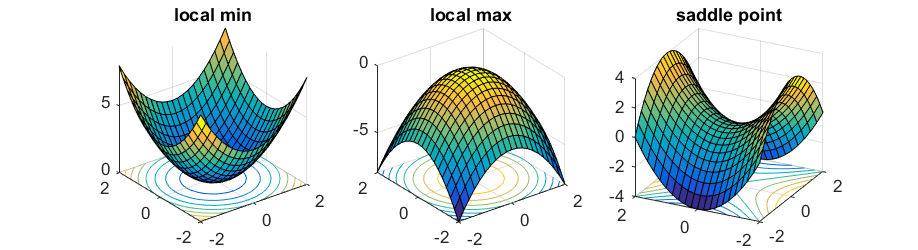
\includegraphics[width=5in]{img/minmaxsaddle.png} 
\end{figure}
\end{frame}

\begin{frame}
\frametitle{Local optimality conditions}
\begin{small}
Let $f: D \subset\R^n \rightarrow \R$ twice continuously differentiable ($f \in C^2$).

\textcolor{blue}{The Hessian matrix} of $f$ at point ${\bf x}$ is defined as:
$$
H_f({\bf x})=\left(f_{x_i x_j}({\bf x})\right)_{1 \leq i,j \leq n}.
$$
Observe that the Hessian matrix is always \textcolor{blue}{symmetric}, as $f \in C^2$.



\textcolor{blue}{Theorem (Sufficient 2nd order condition):} Let ${\bf x}$ be a stationary point of $f$. Then:
\begin{enumerate}
\item If $H_f({\bf x})$ is negative (positive) definite, then ${\bf x}$ is a local
max (min) 
\item If $H_f({\bf x})$ is indefinite, then ${\bf x}$ is a saddle point.

\begin{tiny}Otherwise, we don't know it from this theorem. \end{tiny}
\end{enumerate}

 \textcolor{blue}{Theorem ($n=2$):} Let ${\bf x}$ be a stationary point of $f$. Then:
\begin{enumerate}
\item If $\vert H_f({\bf x})\vert >0$ \begin{tiny}(that is, $f_{xx}({\bf x})f_{yy}({\bf x})>f_{xy}^2({\bf x})$) \end{tiny}, then:
\begin{itemize}
\item If $f_{xx}({\bf x})<0$ or $f_{yy}({\bf x})<0$, then ${\bf x}$ is a local max.
\item If $f_{xx}({\bf x})>0$ or $f_{yy}({\bf x})>0$, then ${\bf x}$ is a local min.
\end{itemize}
\item If $\vert H_f({\bf x})\vert <0$, then ${\bf x}$ is a saddle point.

\begin{tiny}Otherwise, we don't know it from this theorem. \end{tiny}
\end{enumerate}



\end{small}
\end{frame}

\begin{frame}
\frametitle{Examples}
\begin{small}
\begin{enumerate}

\item Let $f(x,y)=x^2-y^2-xy$. Since $\nabla f(x,y)=(2x-y, -2y-x)$, the \textcolor{blue}{stationary points} are $(0,0)$. The Hessian matrix is
\begin{equation*}
H_f(x,y)=\begin{pmatrix}
2 & -1 \\
-1 & -2
\end{pmatrix}
\end{equation*}
which is \textcolor{blue}{indefinite}, so $(0,0)$ is a \textcolor{blue}{saddle point}.

\begin{tiny} We will see that in this case the function is neither concave nor convex\end{tiny}

\item Let $f(x,y)=x^2+y^4$. Stationary points: $(0,0)$. The Hessian matrix at $(0,0)$ is
\begin{equation*}
H_f(0,0)=\begin{pmatrix}
2 & 0 \\
0 & 0
\end{pmatrix}
\end{equation*}
which is positive semi-definite
so we cannot conclude from the Hessian matrix but it is clear that $(0,0)$ is \textcolor{blue}{ global minimum} since $f \geq 0$.

\item Let $f(x,y)=x^3+y^3$. Stationary points: $(0,0)$. Similar as 2. but it is clear that $(0,0)$ is a \textcolor{blue}{saddle point}.
\end{enumerate}
\end{small}
\end{frame}




\begin{frame}
\frametitle{Convex domain}
\begin{small}
The domain of a function $f:D \subset \R^n \rightarrow \R$ is said to be \textcolor{blue}{convex} if any line segment joining two points in the domain lies completely within the domain.
\end{small}
\begin{figure}
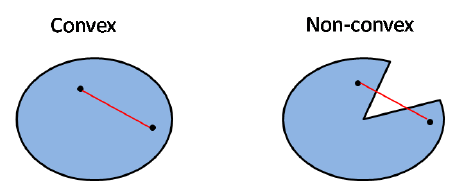
\includegraphics[width=4in]{img/convex_set} 
\end{figure}
\end{frame}



\begin{frame}
\frametitle{Global optimality conditions}
\begin{small}
A function $f:D \subset \R^n \rightarrow \R$ where $D$ is convex is said to be \textcolor{blue}{convex} (resp. \textcolor{blue}{concave}) if the line segment between any two points on the graph of the function lies above (rep. below) or on the graph.
\vskip 12pt
\textcolor{blue}{Theorem:} $f:D \subset \R^n \rightarrow \R$ where $D$ is convex satisfies:
\begin{enumerate}
\item $H_f({\bf x})$ is negative (positive) semi-definite on $D$ $\Leftrightarrow$ $f$ is concave (convex) on $D$
\item $H_f({\bf x})$ is negative (positive) definite on $D$ $\Leftrightarrow$ $f$ is strictly concave (strictly convex) on $D$

\item  If $f$ is convex (concave) on $D$, then all stationary points are global min (max).
\end{enumerate}


\end{small}
\end{frame}



\begin{frame}
\frametitle{Example}
\begin{small}
Let $f(x,y)=2x-y-x^2+xy-y^2$. 
\vskip 8pt
\begin{tiny}Since $\nabla f(x,y)=(2-2x+y, -1+x-2y)$, the \textcolor{blue}{stationary points} are $x=(0,1)$. The Hessian matrix is
\begin{equation*}
H_f(x,y)=\begin{pmatrix}
-2 & 1 \\
1 & -2
\end{pmatrix}
\end{equation*}
which is \textcolor{blue}{negative definite}, so $f$ is strictly concave and $(0,1)$ is a \textcolor{blue}{global maximum}.\end{tiny}
\end{small}
\begin{figure}
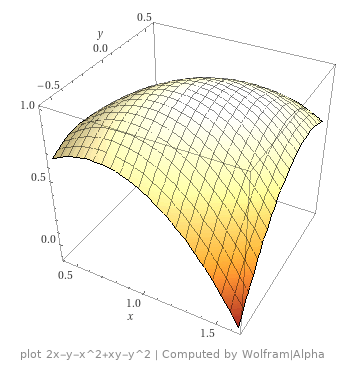
\includegraphics[width=2in]{img/plotxy} 
\end{figure}
\end{frame}

\begin{frame}
\frametitle{Economic example}
\begin{small}
 \textcolor{blue}{Example:} A firm can sell each piece of product $X/Y$ for $45/55$ euros. The revenue is $R(x,y)=45x+55y$. The production cost is
$$
C(x,y)=300+x^2+1.5 y^2-25 x- 35 y.$$ 
The total profit is
$$
f(x,y)=R(x,y)-C(x,y).
$$
We want to know the \textcolor{blue}{maximum profit} the firm can make. We first find the stationary points of $f$:
$$
f_x=-2x+70=0, \; \; f_y=-3y+90=0 \quad \Longrightarrow {\bf  x}=(35,30).
$$
We next check the 2nd order conditions:
since $H_f({\bf x})$ is negative definite, ${\bf x}$ is a local max of $f$.  Is it  a global  max? Yes, since $H_f({\bf x})$ is negative definite for all ${\bf x}$ so strictly concave. The maximal profit is $f(35,30)=2275$.


\end{small}
\end{frame}



\begin{frame}
\frametitle{Method of least squares}
\begin{small}
 Consider a linear system of equations $A {\bf x}={\bf b}$ that has \textcolor{blue}{no solution}.


\begin{tiny}That is, ${\bf b}$ does not belong to the span of columns of $A$\end{tiny}

\vskip 12pt
The solutions $\hat{{\bf x}}$ that make $\vert {\bf b}-A \hat{{\bf x}} \vert$ minimal are called \textcolor{blue}{least square solutions}.

\begin{figure}
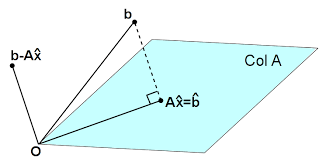
\includegraphics[width=2in]{img/least_squares} 
\end{figure}

\begin{tiny} This is equivalent to find the \textcolor{blue}{orthogonal projection} of ${\bf b}$ onto the span of the columns of $A$ \end{tiny}


\end{small}
\end{frame}

\begin{frame}
\frametitle{Method of least squares}
\begin{small}
The solution is $\hat{{\bf x}}$ is such that
$$
\langle A\hat{{\bf x}}-{\bf b},  A{\bf x}\rangle=0, \quad \text{ for all } {\bf x}.
$$

 This is equivalent to
$$
(A\hat{{\bf x}}-{\bf b})^T A{\bf x}=(\hat{{\bf  x}}' A' A -{\bf b}' A ) {\bf x}=0,
$$
for all ${\bf x}$.
\vskip 10pt

Therefore, $\hat{{\bf x}}$ is the solution to the linear system of equations
$$
A' {\bf b}= A'  A \hat{{\bf x}}.
$$

\begin{tiny} This system has a unique solution if and only if the columns of $A$ are linearly independent. In this case, 
$$
\hat{{\bf  x}}=(A' A)^{-1} A' {\bf b}.
$$
\end{tiny}


\end{small}
\end{frame}



\begin{frame}
\frametitle{Linear fit }
\begin{small}
Assume that we have $n$ \textcolor{blue}{measurements}
${\bf x}=(x_1,...,x_n)$ and ${\bf y}=(y_1,...,y_n)$ of two variables $x$ and $y$, respectively.
\vskip 12pt
We want to find the line $y=ax+b$ that describes the relation between both variables using the least square approximation. That is, 
\begin{equation*}
\begin{pmatrix}
x_1 & 1\\
x_2 & 1 \\
\vdots & \vdots \\
x_n& 1 
\end{pmatrix} \begin{pmatrix}
a\\
b  
\end{pmatrix} =\begin{pmatrix}
y_1\\
y_2 \\
\vdots\\
y_n 
\end{pmatrix}
\end{equation*} 

In this case, the solution to the linear system $
A' {\bf b}= A'  A \hat{{\bf  x}}
$ is
\begin{equation*} \begin{split}
a&=\frac{n \sum_{i=1}^n x_i y_i-\left(\sum_{i=1}^n x_i\right) \left( \sum_{i=1}^n y_i\right)}{n \sum_{i=1}^n x_i^2-\left( \sum_{i=1}^n x_i\right)^2} \\
b&=\frac{\sum_{i=1}^n y_i-a \sum_{i=1}^n x_i}{n}
\end{split}
\end{equation*}


\end{small}
\end{frame}

\begin{frame}
\frametitle{Linear  fit}
\begin{figure}
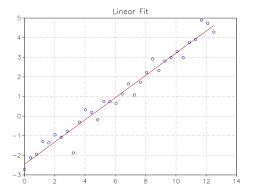
\includegraphics[width=3in]{img/linear_fit} 
\end{figure}
\end{frame}

\begin{frame}
\frametitle{Polynomial fit }
\begin{small}
Assume that we have $n$ \textcolor{blue}{measurements}
${\bf x}=(x_1,...,x_n)$ and ${\bf y}=(y_1,...,y_n)$ of two variables $x$ and $y$, respectively.
\vskip 12pt
 We want to find the polynomial of degree $m$, $y=c_0+c_1 x+c_2 x^2+\cdots+c_m x^m$ that describes the relation between both variables.
\vskip 12pt
Here $A$ is the $n \times m+1$ matrix of a column of ones, the observations ${\bf x}$, ${\bf x}^2, \ldots,
{\bf x}^m$.  The vector ${\bf b}$ is the vector ${\bf y}$, and the least square solution is $(c_0, c_1, \ldots, c_m)$.
\vskip 12pt
Again we need to solve the system of equations $
A' {\bf b}= A'  A \hat{{\bf x}}.
$ 


\end{small}
\end{frame}

\begin{frame}
\frametitle{Example: quadratic fit }
\begin{small}
 We want to find the  best  quadratic polynomial that  fits  the data
${\bf x}=(-1, -0.5, 0, 0.5, 1)$ and ${\bf y}=(1, 0.5, 0, 0.5, 2)$.
\vskip 12pt
 Here $m=2$, $n=5$, 
\begin{equation*}
A=\begin{pmatrix}
1 & -1 & 1\\
1 & -0.5 & 0.25 \\
1 & 0 & 0 \\
1& 0.5 &0.25 \\
1& 1 & 1
\end{pmatrix} 
\end{equation*} 
and
\begin{equation*}
A'  A=\begin{pmatrix}
5 & 0 & 2.5\\
0 & 2.5 & 0 \\
2.5 & 0 & 2.125 
\end{pmatrix} \quad 
A' {\bf b}=\begin{pmatrix}
4\\
1 \\
3.25
\end{pmatrix} 
\end{equation*}

The solution to this system is the  polynomial  $0.0857+0.4x+1.4286 x^2$.


\end{small}
\end{frame}

\begin{frame}
\frametitle{Example:quadratic  fit}
\begin{small}We plot the polynomial $0.0857+0.4x+1.4286 x^2$ and the data.\end{small}
\begin{figure}
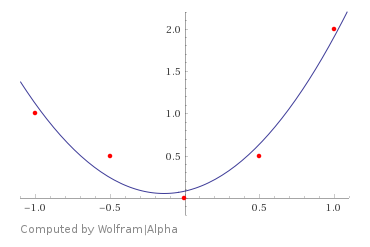
\includegraphics[width=3in]{img/least_squares2} 
\end{figure}
\end{frame}
\end{document}

